\documentclass[]{book}
\usepackage{lmodern}
\usepackage{amssymb,amsmath}
\usepackage{ifxetex,ifluatex}
\usepackage{fixltx2e} % provides \textsubscript
\ifnum 0\ifxetex 1\fi\ifluatex 1\fi=0 % if pdftex
  \usepackage[T1]{fontenc}
  \usepackage[utf8]{inputenc}
\else % if luatex or xelatex
  \ifxetex
    \usepackage{mathspec}
  \else
    \usepackage{fontspec}
  \fi
  \defaultfontfeatures{Ligatures=TeX,Scale=MatchLowercase}
\fi
% use upquote if available, for straight quotes in verbatim environments
\IfFileExists{upquote.sty}{\usepackage{upquote}}{}
% use microtype if available
\IfFileExists{microtype.sty}{%
\usepackage{microtype}
\UseMicrotypeSet[protrusion]{basicmath} % disable protrusion for tt fonts
}{}
\usepackage{hyperref}
\hypersetup{unicode=true,
            pdftitle={An Introduction to Statistical Learning},
            pdfauthor={Steven Golovkine},
            pdfborder={0 0 0},
            breaklinks=true}
\urlstyle{same}  % don't use monospace font for urls
\usepackage{natbib}
\bibliographystyle{apalike}
\usepackage{color}
\usepackage{fancyvrb}
\newcommand{\VerbBar}{|}
\newcommand{\VERB}{\Verb[commandchars=\\\{\}]}
\DefineVerbatimEnvironment{Highlighting}{Verbatim}{commandchars=\\\{\}}
% Add ',fontsize=\small' for more characters per line
\usepackage{framed}
\definecolor{shadecolor}{RGB}{248,248,248}
\newenvironment{Shaded}{\begin{snugshade}}{\end{snugshade}}
\newcommand{\AlertTok}[1]{\textcolor[rgb]{0.94,0.16,0.16}{#1}}
\newcommand{\AnnotationTok}[1]{\textcolor[rgb]{0.56,0.35,0.01}{\textbf{\textit{#1}}}}
\newcommand{\AttributeTok}[1]{\textcolor[rgb]{0.77,0.63,0.00}{#1}}
\newcommand{\BaseNTok}[1]{\textcolor[rgb]{0.00,0.00,0.81}{#1}}
\newcommand{\BuiltInTok}[1]{#1}
\newcommand{\CharTok}[1]{\textcolor[rgb]{0.31,0.60,0.02}{#1}}
\newcommand{\CommentTok}[1]{\textcolor[rgb]{0.56,0.35,0.01}{\textit{#1}}}
\newcommand{\CommentVarTok}[1]{\textcolor[rgb]{0.56,0.35,0.01}{\textbf{\textit{#1}}}}
\newcommand{\ConstantTok}[1]{\textcolor[rgb]{0.00,0.00,0.00}{#1}}
\newcommand{\ControlFlowTok}[1]{\textcolor[rgb]{0.13,0.29,0.53}{\textbf{#1}}}
\newcommand{\DataTypeTok}[1]{\textcolor[rgb]{0.13,0.29,0.53}{#1}}
\newcommand{\DecValTok}[1]{\textcolor[rgb]{0.00,0.00,0.81}{#1}}
\newcommand{\DocumentationTok}[1]{\textcolor[rgb]{0.56,0.35,0.01}{\textbf{\textit{#1}}}}
\newcommand{\ErrorTok}[1]{\textcolor[rgb]{0.64,0.00,0.00}{\textbf{#1}}}
\newcommand{\ExtensionTok}[1]{#1}
\newcommand{\FloatTok}[1]{\textcolor[rgb]{0.00,0.00,0.81}{#1}}
\newcommand{\FunctionTok}[1]{\textcolor[rgb]{0.00,0.00,0.00}{#1}}
\newcommand{\ImportTok}[1]{#1}
\newcommand{\InformationTok}[1]{\textcolor[rgb]{0.56,0.35,0.01}{\textbf{\textit{#1}}}}
\newcommand{\KeywordTok}[1]{\textcolor[rgb]{0.13,0.29,0.53}{\textbf{#1}}}
\newcommand{\NormalTok}[1]{#1}
\newcommand{\OperatorTok}[1]{\textcolor[rgb]{0.81,0.36,0.00}{\textbf{#1}}}
\newcommand{\OtherTok}[1]{\textcolor[rgb]{0.56,0.35,0.01}{#1}}
\newcommand{\PreprocessorTok}[1]{\textcolor[rgb]{0.56,0.35,0.01}{\textit{#1}}}
\newcommand{\RegionMarkerTok}[1]{#1}
\newcommand{\SpecialCharTok}[1]{\textcolor[rgb]{0.00,0.00,0.00}{#1}}
\newcommand{\SpecialStringTok}[1]{\textcolor[rgb]{0.31,0.60,0.02}{#1}}
\newcommand{\StringTok}[1]{\textcolor[rgb]{0.31,0.60,0.02}{#1}}
\newcommand{\VariableTok}[1]{\textcolor[rgb]{0.00,0.00,0.00}{#1}}
\newcommand{\VerbatimStringTok}[1]{\textcolor[rgb]{0.31,0.60,0.02}{#1}}
\newcommand{\WarningTok}[1]{\textcolor[rgb]{0.56,0.35,0.01}{\textbf{\textit{#1}}}}
\usepackage{longtable,booktabs}
\usepackage{graphicx,grffile}
\makeatletter
\def\maxwidth{\ifdim\Gin@nat@width>\linewidth\linewidth\else\Gin@nat@width\fi}
\def\maxheight{\ifdim\Gin@nat@height>\textheight\textheight\else\Gin@nat@height\fi}
\makeatother
% Scale images if necessary, so that they will not overflow the page
% margins by default, and it is still possible to overwrite the defaults
% using explicit options in \includegraphics[width, height, ...]{}
\setkeys{Gin}{width=\maxwidth,height=\maxheight,keepaspectratio}
\IfFileExists{parskip.sty}{%
\usepackage{parskip}
}{% else
\setlength{\parindent}{0pt}
\setlength{\parskip}{6pt plus 2pt minus 1pt}
}
\setlength{\emergencystretch}{3em}  % prevent overfull lines
\providecommand{\tightlist}{%
  \setlength{\itemsep}{0pt}\setlength{\parskip}{0pt}}
\setcounter{secnumdepth}{5}
% Redefines (sub)paragraphs to behave more like sections
\ifx\paragraph\undefined\else
\let\oldparagraph\paragraph
\renewcommand{\paragraph}[1]{\oldparagraph{#1}\mbox{}}
\fi
\ifx\subparagraph\undefined\else
\let\oldsubparagraph\subparagraph
\renewcommand{\subparagraph}[1]{\oldsubparagraph{#1}\mbox{}}
\fi

%%% Use protect on footnotes to avoid problems with footnotes in titles
\let\rmarkdownfootnote\footnote%
\def\footnote{\protect\rmarkdownfootnote}

%%% Change title format to be more compact
\usepackage{titling}

% Create subtitle command for use in maketitle
\providecommand{\subtitle}[1]{
  \posttitle{
    \begin{center}\large#1\end{center}
    }
}

\setlength{\droptitle}{-2em}

  \title{An Introduction to Statistical Learning}
    \pretitle{\vspace{\droptitle}\centering\huge}
  \posttitle{\par}
    \author{Steven Golovkine}
    \preauthor{\centering\large\emph}
  \postauthor{\par}
      \predate{\centering\large\emph}
  \postdate{\par}
    \date{2019-11-01}

\usepackage{booktabs}

\begin{document}
\maketitle

{
\setcounter{tocdepth}{1}
\tableofcontents
}
\hypertarget{introduction}{%
\chapter{Introduction}\label{introduction}}

This book aims to provide my results to the different exercises of \emph{An Introduction to Statistical Learning, with Application in R}, by James, Witten, Hastie and Tibshirani \citep{James2013}. The applied exercises will be solved using the packages from the tidyverse (\url{https://www.tidyverse.org}) when it is possible.

This book is compiled using R Markdown and \textbf{bookdown} (\url{https://github.com/rstudio/bookdown}).

\hypertarget{overview}{%
\chapter{An Overview of Statistical Learning}\label{overview}}

\hypertarget{conceptual-exercises}{%
\section{Conceptual Exercises}\label{conceptual-exercises}}

\hypertarget{exercise-1.}{%
\subsection{Exercise 1.}\label{exercise-1.}}

This exercise is about \emph{flexible} and \emph{inflexible} statistical learning methods. First, let's recall what are the differences between these methods. The aim of statistical learning is to estimate a function \(f\) such that \(f\) is a link between the input \(X\) and the output \(Y\). A \emph{flexible} model means that we do not assume a particular form for \(f\). So, an advantage of such models is to generally provide a better fit to the data (however, be careful with the overfitting) but the number of parameters to estimate is usually large. At the contrary, an \emph{inflexible} model has less parameters but we have to prespecified a particular form for the data (for example linear), even if it poorly fits the data.

\begin{itemize}
\tightlist
\item
  \emph{Question (a)}
\end{itemize}

The case of sample size \(n\) extremely large and number of predictors \(p\) small is the ideal case in statistical learning. A flexible method should perform very well in this case. The flexible method will tend to reduce the bias and won't be too sensitive to the noise thanks to the large size of the sample.

\begin{itemize}
\tightlist
\item
  \emph{Question (b)}
\end{itemize}

The case of sample size \(n\) small and number of predictors \(p\) very large refers to the high dimensional settings. An inflexible method should show better performance than a flexible one in this case. Here, the trade-off between bias and variance is very important. We allow some bias by using an inflexible model with the hope to reduce a lot the noise in the data.

\begin{itemize}
\tightlist
\item
  \emph{Question (c)}
\end{itemize}

In the case of highly non-linear relationship between predictors and reponse, a flexible model will perform better than an inflexible one. In case of inflexible model, we set a particular form for \(f\) and we usually can not specified a function for \(f\) if \(f\) is highly non-linear.

\begin{itemize}
\tightlist
\item
  \emph{Question (d)}
\end{itemize}

If the variance of the error terms is extremely high, an inflexible model will perform better than a flexible one. Because, if we set a flexible method, the function \(f\) will tend to follow the error and thus will overfit.

\hypertarget{exercise-2.}{%
\subsection{Exercise 2.}\label{exercise-2.}}

This exercise is about the difference between \emph{regression} and \emph{classification} problems and the \emph{inference} or \emph{prediction} purposes. Let's recall what these different terms mean. A \emph{regression} task is done when we try to infer or predict an output which takes continuous values. A \emph{classification} task is done when we try to infer or predict an output which takes discrete values. An \emph{inference} purpose consists in the understanding of how the features have an influence on the response, whereas a \emph{prediction} purpose is to find a value of the output variable based on a new realisation of the dependant variables and the knowledge of some features and outputs.

\begin{itemize}
\tightlist
\item
  \emph{Question (a)}
\end{itemize}

This is a regression problem because the CEO salary is a continuous variable. We aim to do inference here (\emph{understanding which factors}). \(n\) is equal to 500 (top 500 firms in the US), \(p\) equals to 3 (profit, number of employees and industry) and the output is the CEO salary.

\begin{itemize}
\tightlist
\item
  \emph{Question (b)}
\end{itemize}

This is a classification problem because the output varible is discrete (\emph{success} or \emph{failure}). We aim to do prediction (\emph{launching a new product and wish to know whether it will be a success or a failure}). \(n\) is equal to 20, \(p\) equals to 13 (price charged for the product, marketing budget, competition price, and ten other variables) and the output variable is \emph{success or failure}.

\begin{itemize}
\tightlist
\item
  \emph{Question (c)}
\end{itemize}

This is a regression problem because the \% change in the US dollar is continuous. We aim to do prediction (\emph{We are interesting in predicting}). \(n\) is equal to 52 (number of week in 2012), \(p\) equals to 3 (the \% change in the US market, the \% change in the British market, and the \% change in the German market) and the output variable is the \% change in the dollar.

\hypertarget{exercise-3.}{%
\subsection{Exercise 3.}\label{exercise-3.}}

This exercise is about the bias-variance decomposition of the mean square error.

Consider the following model: \(y = f(x) + \epsilon\). We denote by \(\widehat{y}\) and \(\widehat{f}\) the estimation of \(y\) and \(f\). The mean square error is:

\[MSE = \mathbb{E}\left[(\widehat{y} - y)^2\right].\]

As a more complex model leads to a better estimation of the function \(f\), the training error decreases as the model complexity increases. The MSE can be decomposed into three terms: variance, squared bias and irreducible error. ``Variance refers to the amount by which \(\widehat{f}\) would change if we estimated it using a different training data set.'' So, the variance increases with the model complexity because a complex model is very flexible and gives a different function for each training data set. Conversely, the bias decreases with the model complexity because such a model will fit perfectly the data. The irreducible error is equal to \(Var(\epsilon)\). The test error has a U-shape because it is the sum of the three previous curves.

\begin{figure}

{\centering 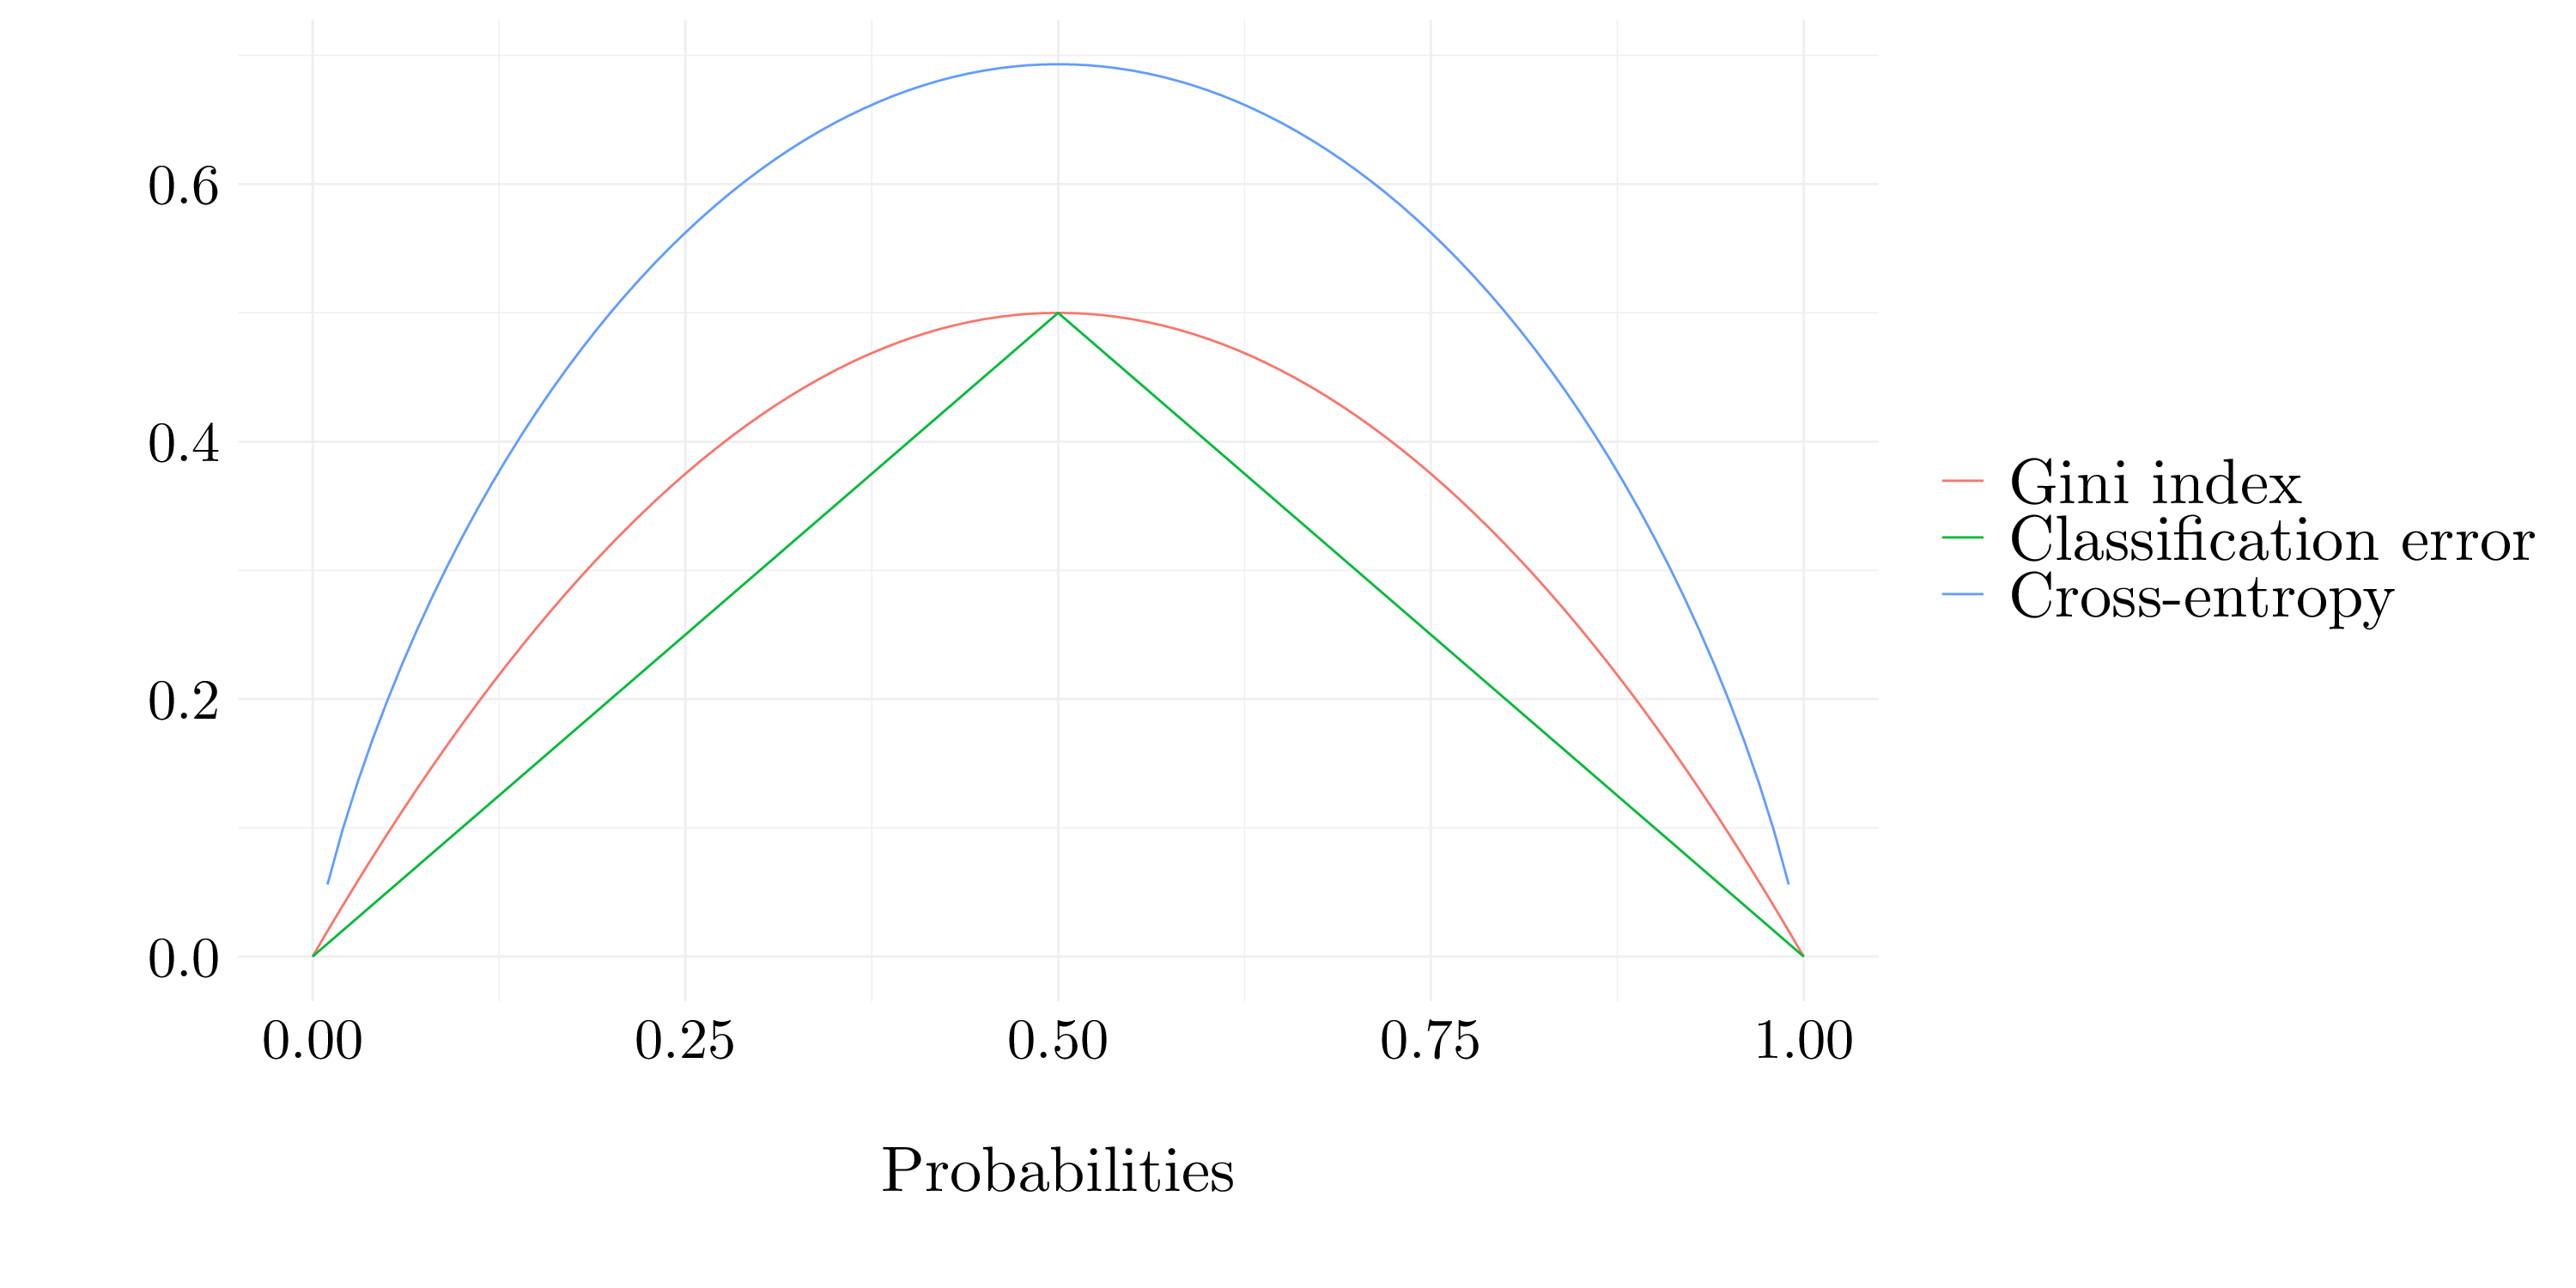
\includegraphics{ISRL_files/figure-latex/ex3-1} 

}

\caption{Model complexity.}\label{fig:ex3}
\end{figure}

\hypertarget{exercise-4.}{%
\subsection{Exercise 4.}\label{exercise-4.}}

This exercise is about giving examples of real-life applications of statistical learning.

\protect\hypertarget{fig:ml_appli}{}{}

From Armando Arroyo GeekStyle on Linkedin.

\hypertarget{exercise-5.}{%
\subsection{Exercise 5.}\label{exercise-5.}}

This exercise is about the difference between flexible and non-flexible statistical learning methods.

A very flexible method has for main advantage over a less flexible methods the large number of functional forms that it can take. It shows two majors drawbacks: the first one is the number of parameters to fit (usually, way more larger than the non-flexible methods) and the second one, its propension to overfit the data. Moreover, they can exhibit less interpretability.

We can prefer a less flexible approach when we want to do inference of the dataset because of the interpretability of such models. However, when the goal is prediction, we may use very flexible methods in order to (hopefully) have better results. The choice of between a very flexible and a less flexible method refers closely with the bias-variance tradeoff. In general, a very flexible one will lead to small bias, large variance and a less flexible one to large bias, small variance.

\hypertarget{exercise-6.}{%
\subsection{Exercise 6.}\label{exercise-6.}}

This exercise is about the difference between parametric and non-parametric approaches.

Consider the following model: \(Y = f(X) + \epsilon\). We aim to estimate the function \(f\). For the parametric approaches, we assume a particular form for \(f\), linear for example, and then, estimate some parameters. However, if the form we assume is not the right one, our estimate won't be very accurate. At the opposite, non-parametric approaches do not assume a particular form for \(f\). So, the estimate of \(f\) will be close to the true functional form of \(f\). But, we need a lot of data (compare to parametric approches) to obtain an accurate estimate of \(f\).

\hypertarget{exercise-7.}{%
\subsection{Exercise 7.}\label{exercise-7.}}

This exercise is an application of \(K\)-nearest neighbors.

\begin{longtable}[]{@{}ccccc@{}}
\caption{Data}\tabularnewline
\toprule
Obs & \(X_1\) & \(X_2\) & \(X_3\) & \(Y\)\tabularnewline
\midrule
\endfirsthead
\toprule
Obs & \(X_1\) & \(X_2\) & \(X_3\) & \(Y\)\tabularnewline
\midrule
\endhead
1 & 0 & 3 & 0 & Red\tabularnewline
2 & 2 & 0 & 0 & Red\tabularnewline
3 & 0 & 1 & 3 & Red\tabularnewline
4 & 0 & 1 & 2 & Green\tabularnewline
5 & -1 & 0 & 1 & Green\tabularnewline
6 & 1 & 1 & 1 & Red\tabularnewline
\bottomrule
\end{longtable}

\begin{itemize}
\tightlist
\item
  \emph{Question (a)}
\end{itemize}

The euclidean distance between to two \(n\)-dimensional vectors \(X\) and \(Y\) is defined by
\[ d(X, Y) = \sqrt{\sum_{i = 1}^n (X_i - Y_i)^2}\]

\begin{longtable}[]{@{}ccccccc@{}}
\toprule
Obs & 1 & 2 & 3 & 4 & 5 & 6\tabularnewline
\midrule
\endhead
\(d(0/i)\) & 3 & 2 & \(\sqrt{10}\) & \(\sqrt{5}\) & \(\sqrt{2}\) & \(\sqrt{3}\)\tabularnewline
\bottomrule
\end{longtable}

\begin{itemize}
\tightlist
\item
  \emph{Question (b)}
\end{itemize}

For \(K = 1\), we classify the test point where the closest observation is. The closest point is the point 5, so the test point will be \emph{Green}.

\begin{itemize}
\tightlist
\item
  \emph{Question (c)}
\end{itemize}

For \(K = 3\), we classify the test point where the three closest observation are. The three closest points are the 2, 5 and 6. Two points are red and one is green, so the test point will be \emph{Red}.

\begin{itemize}
\tightlist
\item
  \emph{Question (d)}
\end{itemize}

If the Bayes decision boundary in this problem is highly non-linear, we would expect the best value for K to be small because the smaller \(K\) is, the more flexible the model is. So, if the model is very flexible, it will adapt to highly non-linear problem.

\hypertarget{applied-exercises}{%
\section{Applied Exercises}\label{applied-exercises}}

\hypertarget{exercise-8.}{%
\subsection{Exercise 8.}\label{exercise-8.}}

This exercise is about the \texttt{College} dataset. It contains 777 observations of 18 variables about the universities and colleges in the United States. For a description of the variables, please refer to the page 54 of the book or in \textbf{R} by typing \texttt{help(College)} after loading the package \texttt{ISLR}.

\begin{itemize}
\tightlist
\item
  \emph{Question (a) and (b)}
\end{itemize}

\begin{Shaded}
\begin{Highlighting}[]
\NormalTok{College <-}\StringTok{ }\KeywordTok{as_tibble}\NormalTok{(College, }\DataTypeTok{rownames =} \OtherTok{NA}\NormalTok{)}
\end{Highlighting}
\end{Shaded}

\begin{itemize}
\tightlist
\item
  \emph{Question (c) i}
\end{itemize}

\begin{Shaded}
\begin{Highlighting}[]
\NormalTok{College }\OperatorTok\StringTok{ }\KeywordTok{summary_df}\NormalTok{() }\OperatorTok\StringTok{ }\KeywordTok{print_summary_df}\NormalTok{()}
\end{Highlighting}
\end{Shaded}

\textbf{Factor variables}

Private

Private

Count

No

212

Yes

565

\textbf{Numeric variables}

Name

NA\_num

Unique

Range

Mean

Variance

Minimum

Q05

Q10

Q25

Q50

Q75

Q90

Q95

Maximum

Apps

0

711

48013.0

3001.64

14978459.53

81.0

329.8

457.6

776.0

1558.0

3624.0

7675.0

11066.2

48094.0

Accept

0

693

26258.0

2018.80

6007959.70

72.0

272.4

361.6

604.0

1110.0

2424.0

4814.2

6979.2

26330.0

Enroll

0

581

6357.0

779.97

863368.39

35.0

118.6

154.0

242.0

434.0

902.0

1903.6

2757.0

6392.0

Top10perc

0

82

95.0

27.56

311.18

1.0

7.0

10.0

15.0

23.0

35.0

50.4

65.2

96.0

Top25perc

0

89

91.0

55.80

392.23

9.0

25.8

30.6

41.0

54.0

69.0

85.0

93.0

100.0

F.Undergrad

0

714

31504.0

3699.91

23526579.33

139.0

509.8

641.0

992.0

1707.0

4005.0

10024.4

14477.8

31643.0

P.Undergrad

0

566

21835.0

855.30

2317798.85

1.0

20.0

35.0

95.0

353.0

967.0

2016.6

3303.6

21836.0

Outstate

0

640

19360.0

10440.67

16184661.63

2340.0

4601.6

5568.8

7320.0

9990.0

12925.0

16552.8

18498.0

21700.0

Room.Board

0

553

6344.0

4357.53

1202743.03

1780.0

2735.8

3051.2

3597.0

4200.0

5050.0

5950.0

6382.0

8124.0

Books

0

122

2244.0

549.38

27259.78

96.0

350.0

400.0

470.0

500.0

600.0

700.0

765.6

2340.0

Personal

0

294

6550.0

1340.64

458425.75

250.0

500.0

600.0

850.0

1200.0

1700.0

2200.0

2488.8

6800.0

PhD

0

78

95.0

72.66

266.61

8.0

43.8

50.6

62.0

75.0

85.0

92.0

95.0

103.0

Terminal

0

65

76.0

79.70

216.75

24.0

52.8

59.0

71.0

82.0

92.0

96.0

98.0

100.0

S.F.Ratio

0

173

37.3

14.09

15.67

2.5

8.3

9.9

11.5

13.6

16.5

19.2

21.0

39.8

perc.alumni

0

61

64.0

22.74

153.56

0.0

6.0

8.0

13.0

21.0

31.0

40.0

46.0

64.0

Expend

0

744

53047.0

9660.17

27266865.64

3186.0

4795.8

5558.2

6751.0

8377.0

10830.0

14841.0

17974.8

56233.0

Grad.Rate

0

81

108.0

65.46

295.07

10.0

37.0

44.6

53.0

65.0

78.0

89.0

94.2

118.0

\begin{itemize}
\tightlist
\item
  \emph{Question (c) ii}
\end{itemize}

\begin{figure}

{\centering 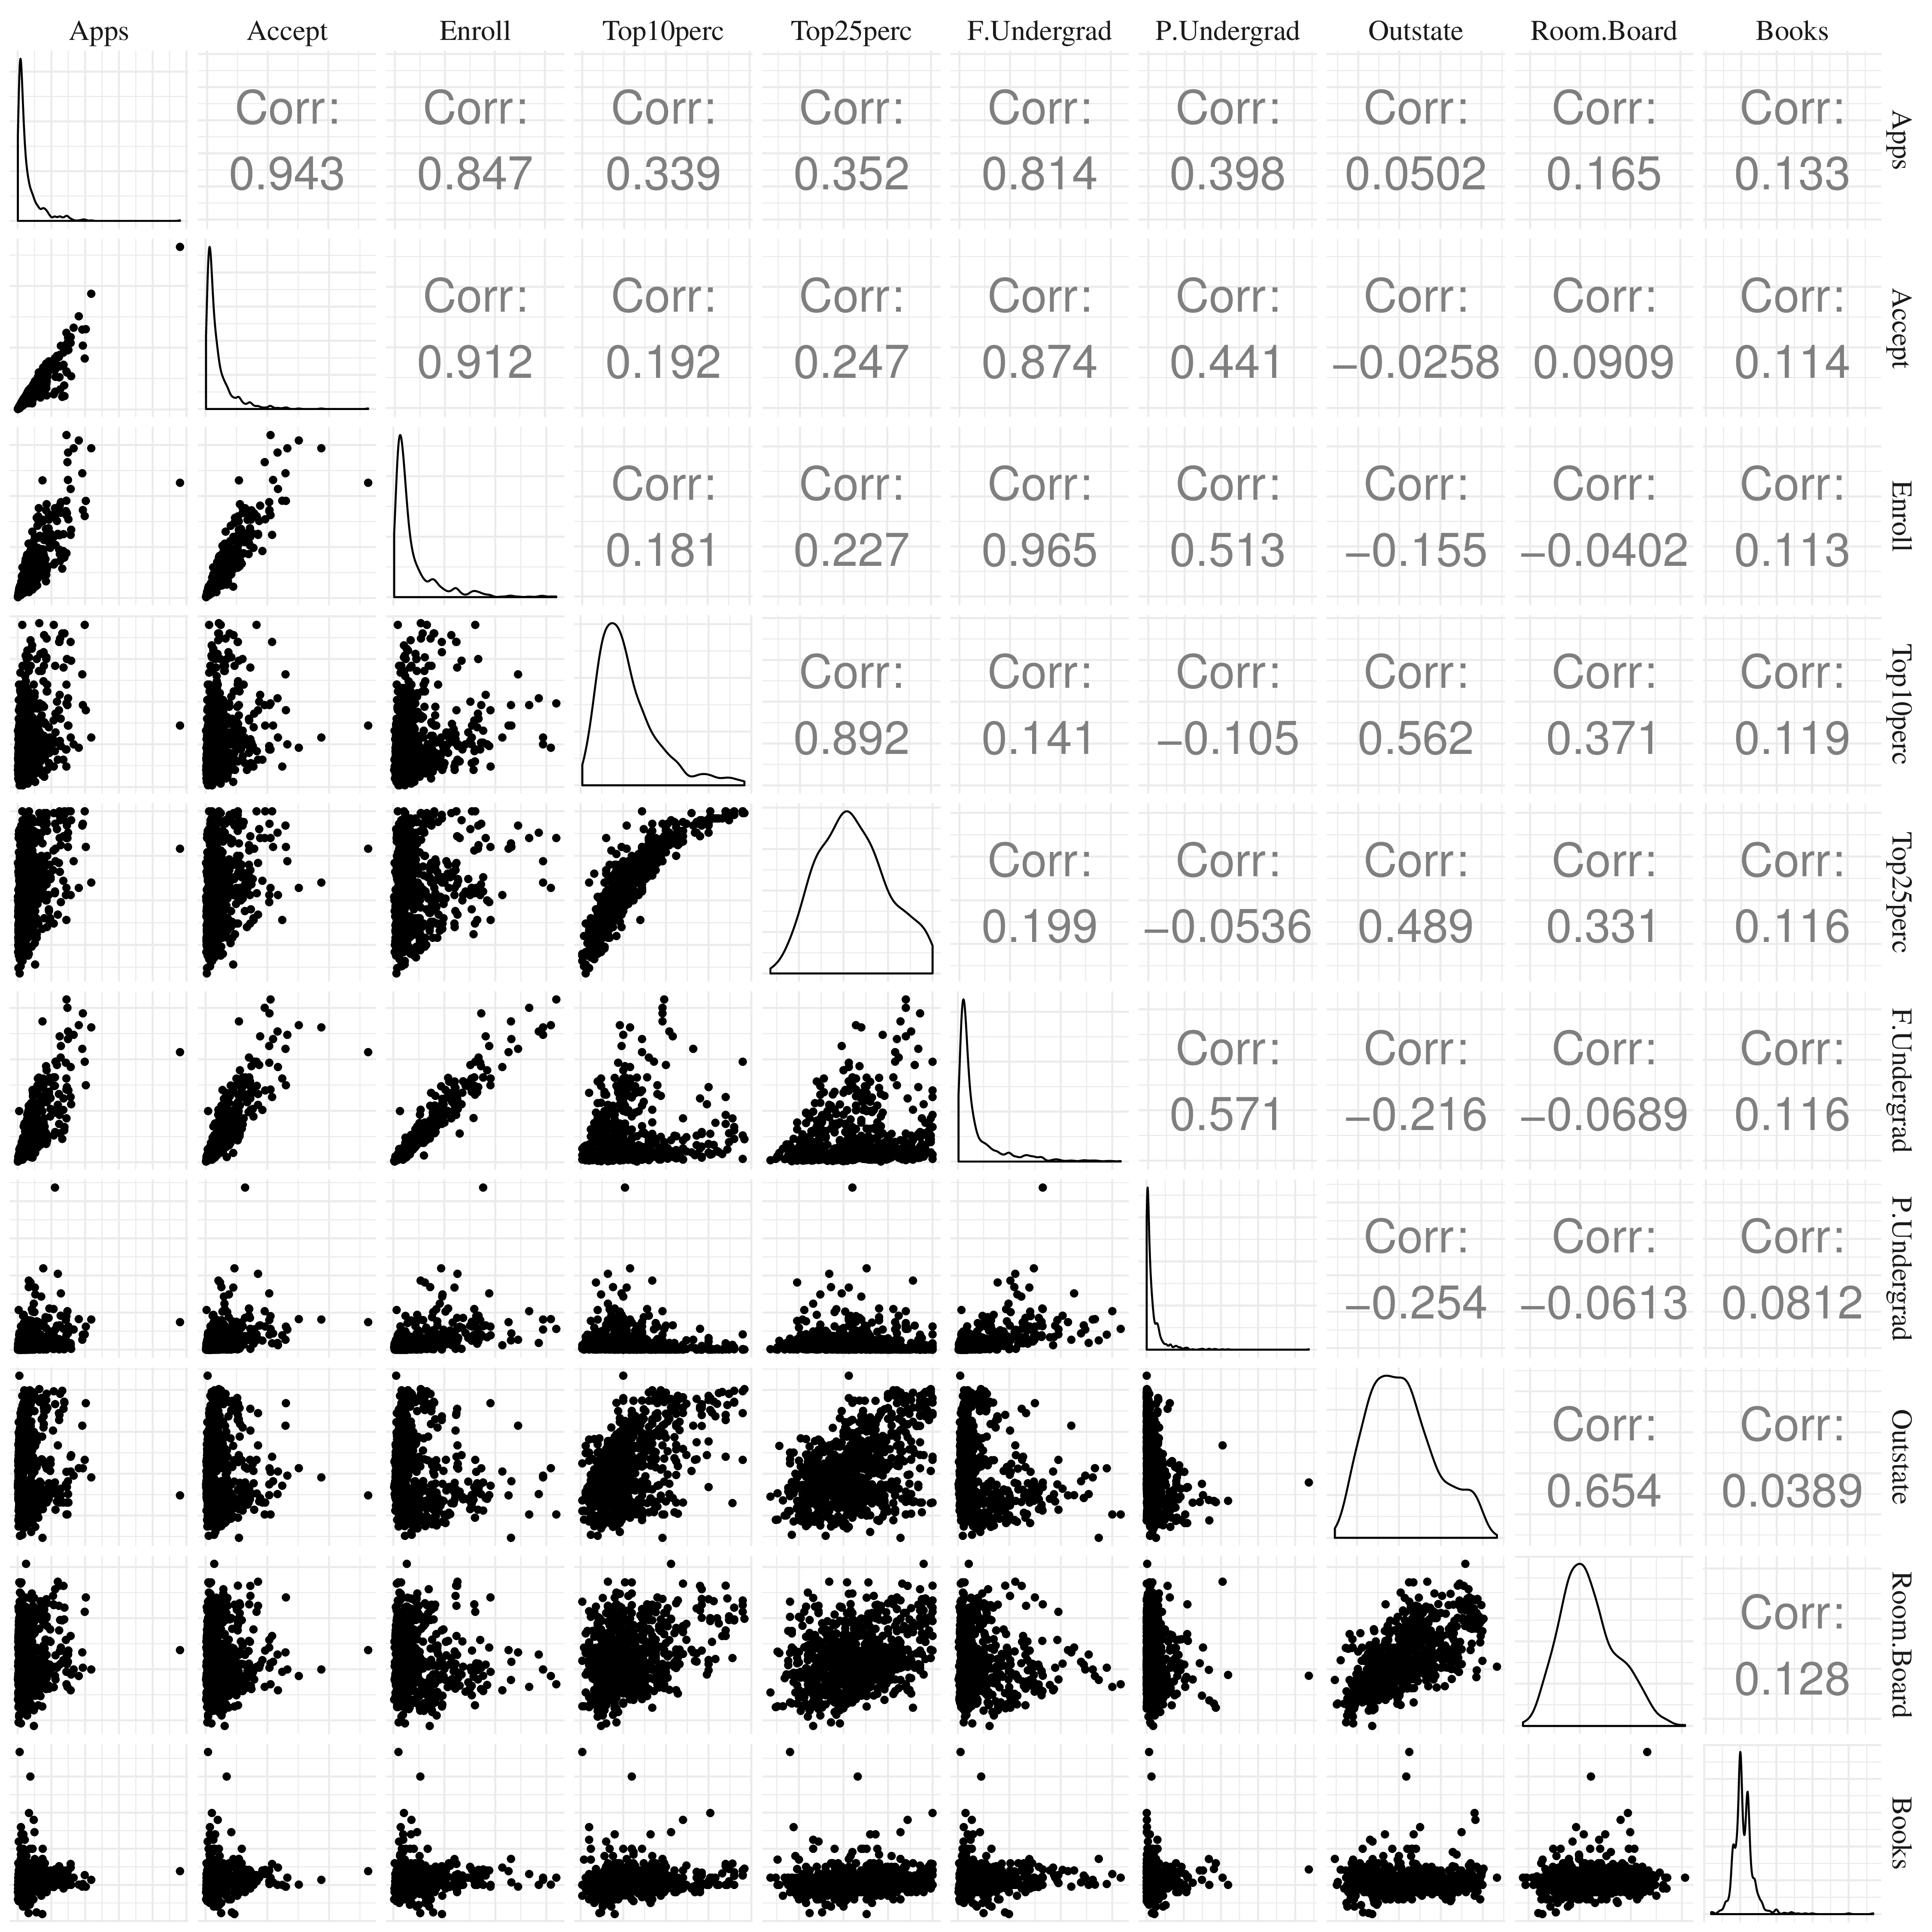
\includegraphics{ISRL_files/figure-latex/ex8cii-1} 

}

\caption{Pair plots.}\label{fig:ex8cii}
\end{figure}

\begin{itemize}
\tightlist
\item
  \emph{Question (c) iii}
\end{itemize}

\begin{figure}

{\centering 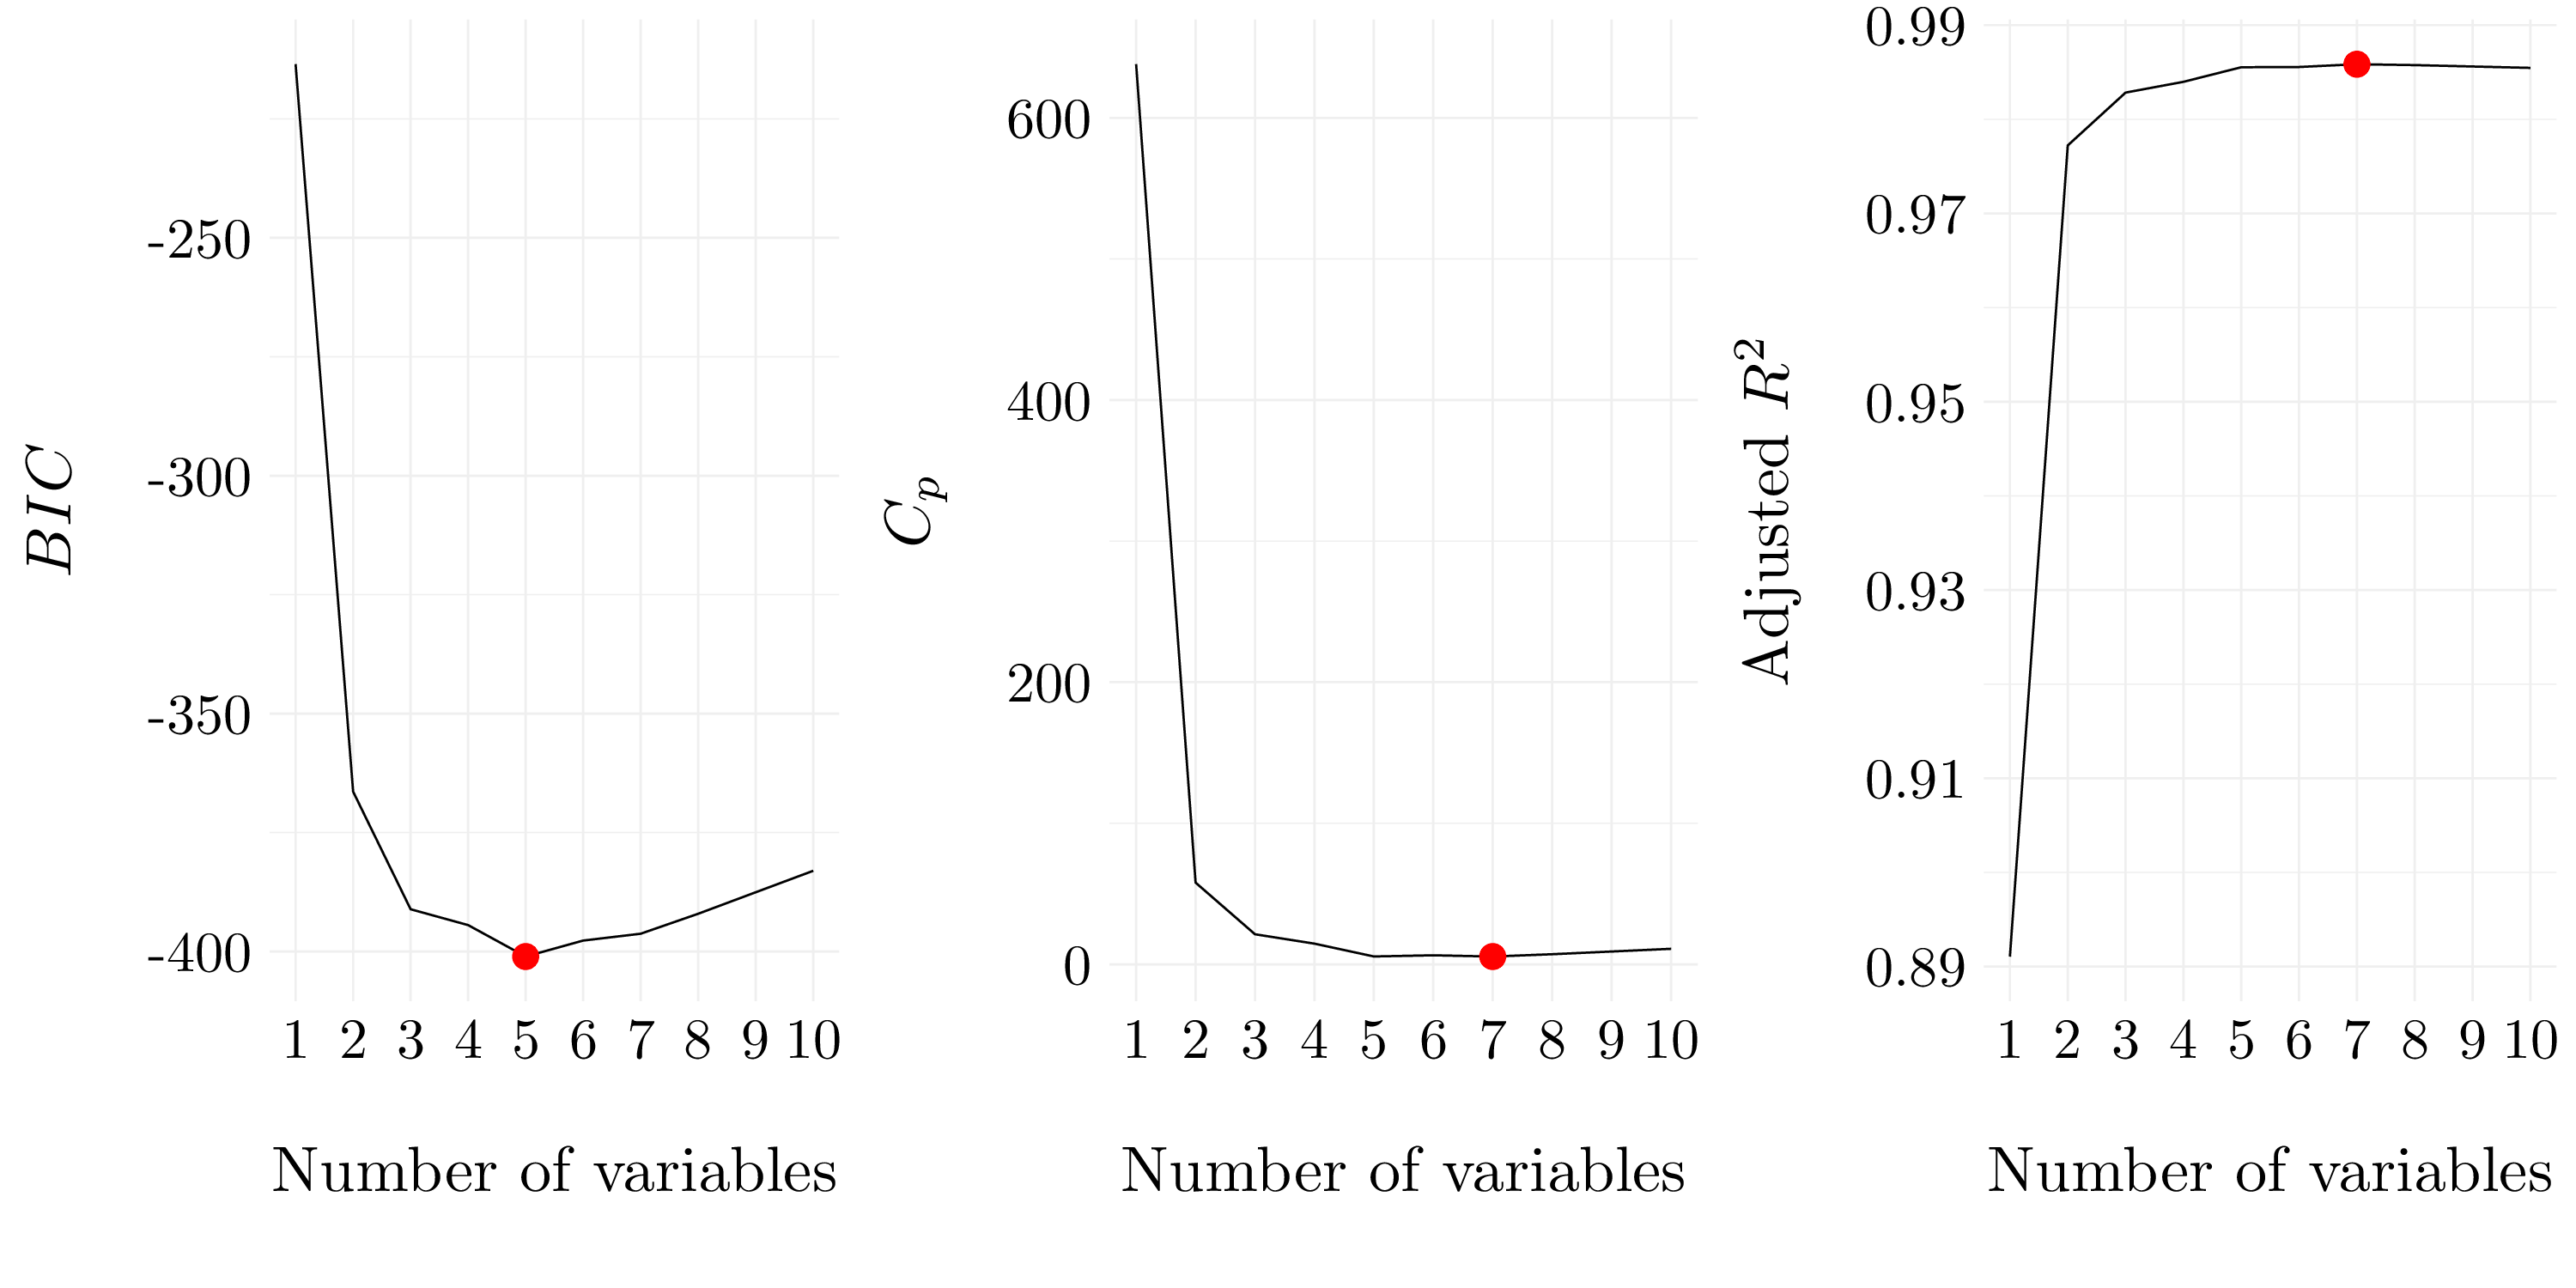
\includegraphics{ISRL_files/figure-latex/ex8ciii-1} 

}

\caption{Boxplots of the variable Outstate by Private.}\label{fig:ex8ciii}
\end{figure}

\begin{itemize}
\tightlist
\item
  \emph{Question (c) iv}
\end{itemize}

\begin{Shaded}
\begin{Highlighting}[]
\NormalTok{College <-}\StringTok{ }\NormalTok{College }\OperatorTok\StringTok{ }\KeywordTok{mutate}\NormalTok{(}\DataTypeTok{Elite =} \KeywordTok{factor}\NormalTok{(Top10perc }\OperatorTok{>}\StringTok{ }\DecValTok{50}\NormalTok{))}
\end{Highlighting}
\end{Shaded}

\begin{Shaded}
\begin{Highlighting}[]
\NormalTok{College }\OperatorTok\StringTok{ }\KeywordTok{select}\NormalTok{(Elite) }\OperatorTok\StringTok{ }\KeywordTok{summary_df}\NormalTok{() }\OperatorTok\StringTok{ }\KeywordTok{print_summary_df}\NormalTok{()}
\end{Highlighting}
\end{Shaded}

\textbf{Factor variables}

Elite

Elite

Count

FALSE

699

TRUE

78

\begin{figure}

{\centering 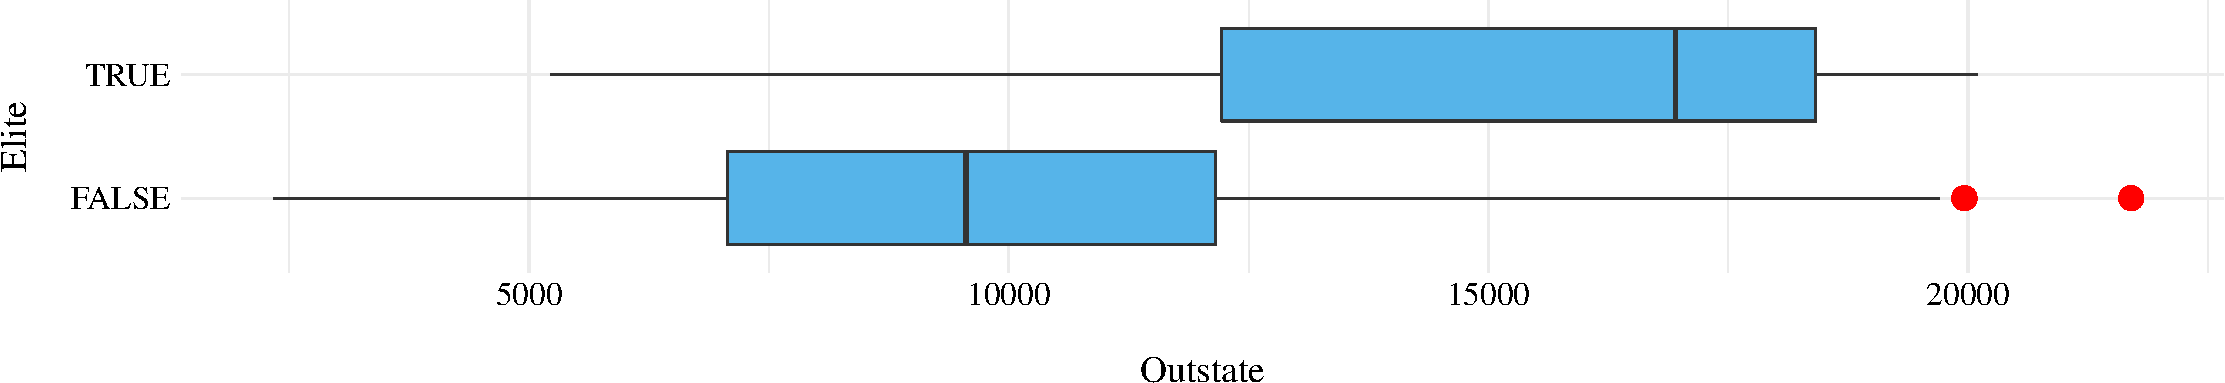
\includegraphics{ISRL_files/figure-latex/ex8civ3-1} 

}

\caption{Boxplots of the variable Outstate vs Elite.}\label{fig:ex8civ3}
\end{figure}

\begin{itemize}
\tightlist
\item
  \emph{Question (c) v}
\end{itemize}

\begin{figure}

{\centering 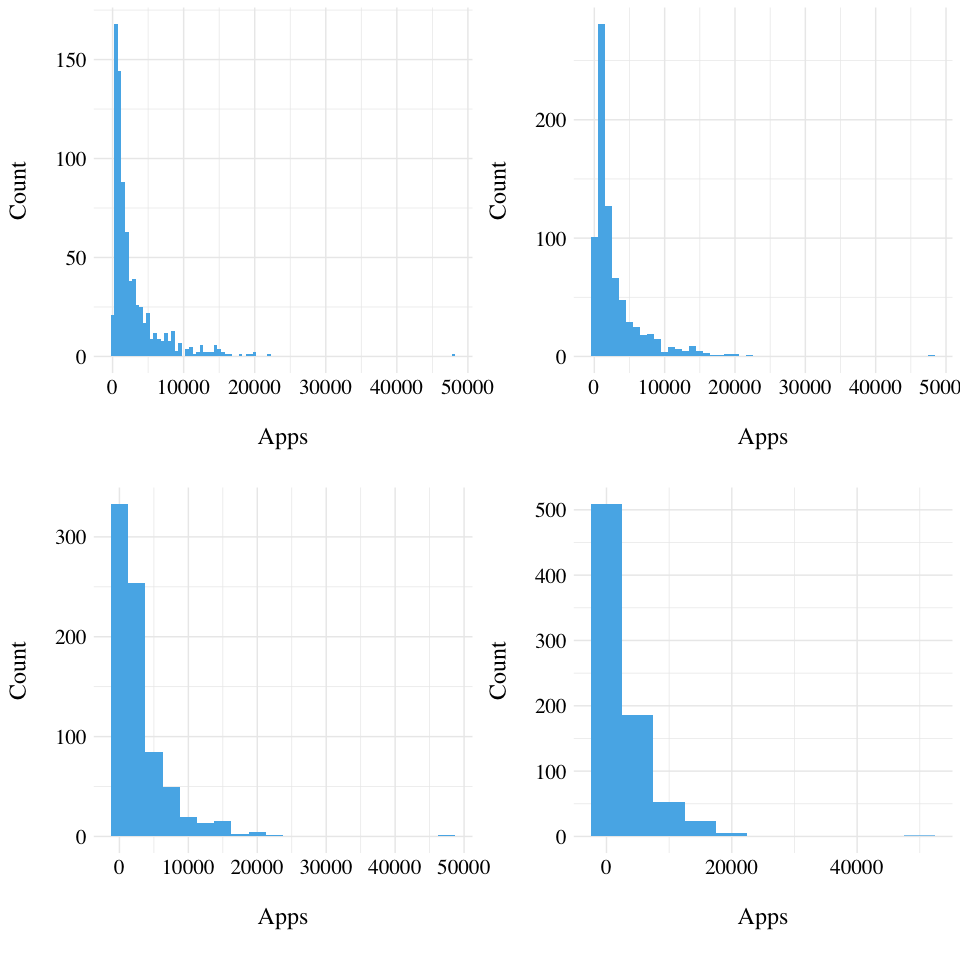
\includegraphics{ISRL_files/figure-latex/ex8cv-1} 

}

\caption{Histograms of the variable Apps for different binwidth.}\label{fig:ex8cv}
\end{figure}

\begin{itemize}
\tightlist
\item
  \emph{Question (c) vi}
\end{itemize}

As a brief summary, we found that there is a huge correlation between the number of full-time undergraduates and the number of applications received, accepted and students enrolled. The price to be enrolled in a private university is in mean twice as the price for a public one. But the variance of the price for the private colleges is very important. Moreover, the maximum value of the price for public universities is almost equal to the mean of the private ones (except outliers). Finally, the elite universities (the ones with new students from top 10\% of high school class) are usually more expensive than the other ones.

\hypertarget{exercise-10.}{%
\subsection{Exercise 10.}\label{exercise-10.}}

This exercise is about the \texttt{Auto} dataset. It contains 392 observations of 9 variables about vehicles. For a description of the variables, please refer to \textbf{R} by typing \texttt{help(Auto)} after loading the package \texttt{ISLR}.

\begin{Shaded}
\begin{Highlighting}[]
\NormalTok{Auto <-}\StringTok{ }\KeywordTok{as_tibble}\NormalTok{(Auto, }\DataTypeTok{rownames =} \OtherTok{NA}\NormalTok{)}
\NormalTok{Auto <-}\StringTok{ }\NormalTok{Auto }\OperatorTok\StringTok{ }\KeywordTok{select}\NormalTok{(}\OperatorTok{-}\NormalTok{name) }\OperatorTok\StringTok{ }
\StringTok{  }\KeywordTok{mutate}\NormalTok{(}\DataTypeTok{cylinders =} \KeywordTok{as.factor}\NormalTok{(cylinders), }\DataTypeTok{year =} \KeywordTok{as.factor}\NormalTok{(year), }\DataTypeTok{origin =} \KeywordTok{as.factor}\NormalTok{(origin))}
\end{Highlighting}
\end{Shaded}

\begin{itemize}
\tightlist
\item
  \emph{Question (a), (b) and (c)}
\end{itemize}

\begin{Shaded}
\begin{Highlighting}[]
\NormalTok{Auto }\OperatorTok\StringTok{ }\KeywordTok{summary_df}\NormalTok{() }\OperatorTok\StringTok{ }\KeywordTok{print_summary_df}\NormalTok{()}
\end{Highlighting}
\end{Shaded}

\textbf{Factor variables}

cylinders

cylinders

Count

3

4

4

199

5

3

6

83

8

103

year

year

Count

70

29

71

27

72

28

73

40

74

26

75

30

76

34

77

28

78

36

79

29

80

27

81

28

82

30

origin

origin

Count

1

245

2

68

3

79

\textbf{Numeric variables}

Name

NA\_num

Unique

Range

Mean

Variance

Minimum

Q05

Q10

Q25

Q50

Q75

Q90

Q95

Maximum

mpg

0

127

37.6

23.45

60.92

9

13.000

14

17.000

22.75

29.000

34.19

37.000

46.6

displacement

0

81

387.0

194.41

10950.37

68

85.000

90

105.000

151.00

275.750

350.00

400.000

455.0

horsepower

0

93

184.0

104.47

1481.57

46

60.550

67

75.000

93.50

126.000

157.70

180.000

230.0

weight

0

346

3527.0

2977.58

721484.71

1613

1931.600

1990

2225.250

2803.50

3614.750

4277.60

4464.000

5140.0

acceleration

0

95

16.8

15.54

7.61

8

11.255

12

13.775

15.50

17.025

19.00

20.235

24.8

\begin{itemize}
\tightlist
\item
  \emph{Question (d)}
\end{itemize}

\begin{Shaded}
\begin{Highlighting}[]
\NormalTok{Auto }\OperatorTok\StringTok{ }\KeywordTok{slice}\NormalTok{(}\OperatorTok{-}\KeywordTok{c}\NormalTok{(}\DecValTok{10}\OperatorTok{:}\DecValTok{85}\NormalTok{)) }\OperatorTok\StringTok{ }\KeywordTok{summary_df}\NormalTok{() }\OperatorTok\StringTok{ }\KeywordTok{print_summary_df}\NormalTok{()}
\end{Highlighting}
\end{Shaded}

\textbf{Factor variables}

cylinders

cylinders

Count

3

3

4

166

5

3

6

71

8

73

year

year

Count

70

9

71

0

72

0

73

39

74

26

75

30

76

34

77

28

78

36

79

29

80

27

81

28

82

30

origin

origin

Count

1

194

2

54

3

68

\textbf{Numeric variables}

Name

NA\_num

Unique

Range

Mean

Variance

Minimum

Q05

Q10

Q25

Q50

Q75

Q90

Q95

Maximum

mpg

0

125

35.6

24.40

61.89

11.0

13.0

15.0

18.00

23.95

30.55

35.4

37.775

46.6

displacement

0

70

387.0

187.24

9935.78

68.0

85.0

90.0

100.25

145.50

250.00

350.0

360.000

455.0

horsepower

0

84

184.0

100.72

1275.12

46.0

60.0

65.0

75.00

90.00

115.00

150.0

170.000

230.0

weight

0

279

3348.0

2935.97

658208.03

1649.0

1934.0

1985.0

2213.75

2792.50

3508.00

4177.5

4391.250

4997.0

acceleration

0

92

16.3

15.73

7.26

8.5

11.4

12.5

14.00

15.50

17.30

19.0

20.475

24.8

\begin{itemize}
\tightlist
\item
  \emph{Question (e)}
\end{itemize}

\begin{figure}

{\centering 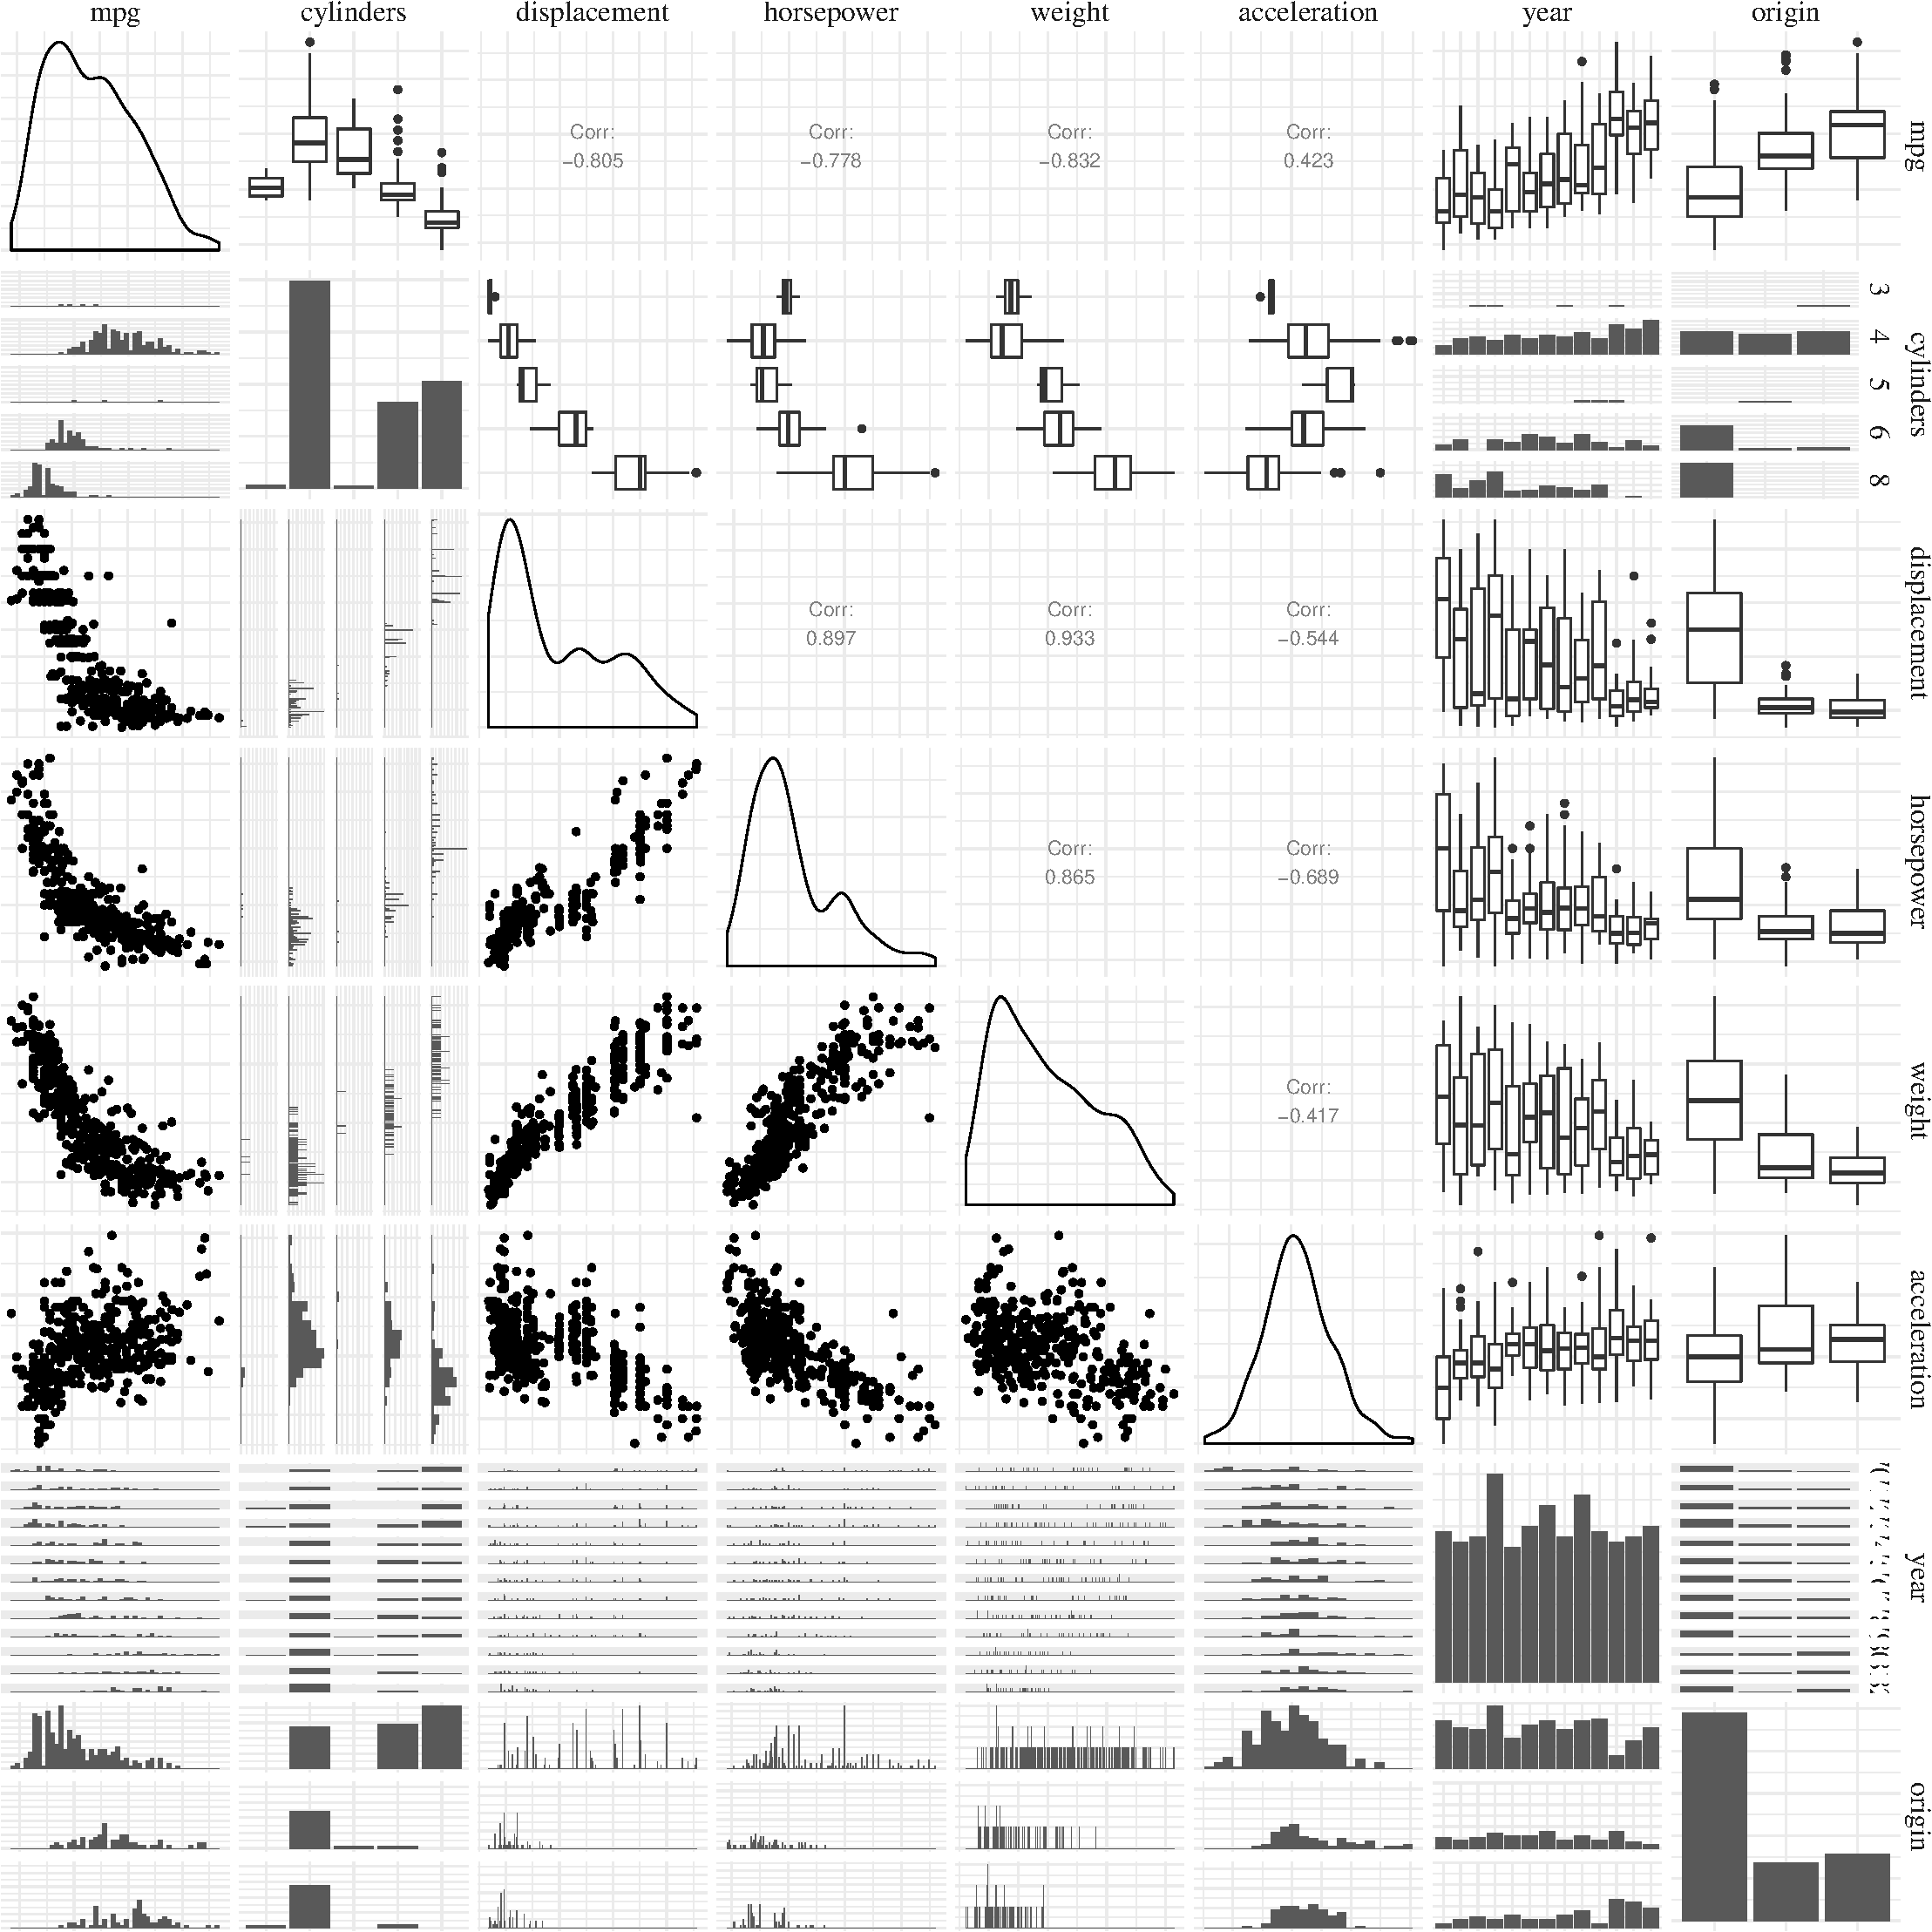
\includegraphics{ISRL_files/figure-latex/ex9e-1} 

}

\caption{Pairs plot}\label{fig:ex9e}
\end{figure}

\begin{itemize}
\tightlist
\item
  \emph{Question (f)}
\end{itemize}

The variables \emph{displacement}, \emph{weight} and \emph{origin} have a huge correlation with the variable to predict, \emph{mpg}. So, this ones could particularly useful for the prediction. The relation between these variables does not seem to be linear but instead in \(\exp(-x)\). Moreover, the miles per gallon look very different depending on the origin of the car.

\hypertarget{exercise-10.-1}{%
\subsection{Exercise 10.}\label{exercise-10.-1}}

This exercise is about the \texttt{Boston} dataset.

\begin{itemize}
\tightlist
\item
  \emph{Question (a)}
\end{itemize}

\begin{Shaded}
\begin{Highlighting}[]
\NormalTok{Boston <-}\StringTok{ }\KeywordTok{as_tibble}\NormalTok{(Boston, }\DataTypeTok{rownames =} \OtherTok{NA}\NormalTok{)}
\NormalTok{Boston <-}\StringTok{ }\NormalTok{Boston }\OperatorTok\StringTok{ }\KeywordTok{mutate}\NormalTok{(}\DataTypeTok{chas =} \KeywordTok{as.logical}\NormalTok{(chas), }\DataTypeTok{rad =} \KeywordTok{as.factor}\NormalTok{(rad))}
\end{Highlighting}
\end{Shaded}

It contains 506 observations of 14 variables about housing values in suburbs of Boston. Each of the observation represents a suburb of Boston. For a description of the variables, please refer to \textbf{R} by typing \texttt{help(Boston)} after loading the package \texttt{MASS}.

\begin{itemize}
\tightlist
\item
  \emph{Question (b)}
\end{itemize}

\begin{figure}
\centering
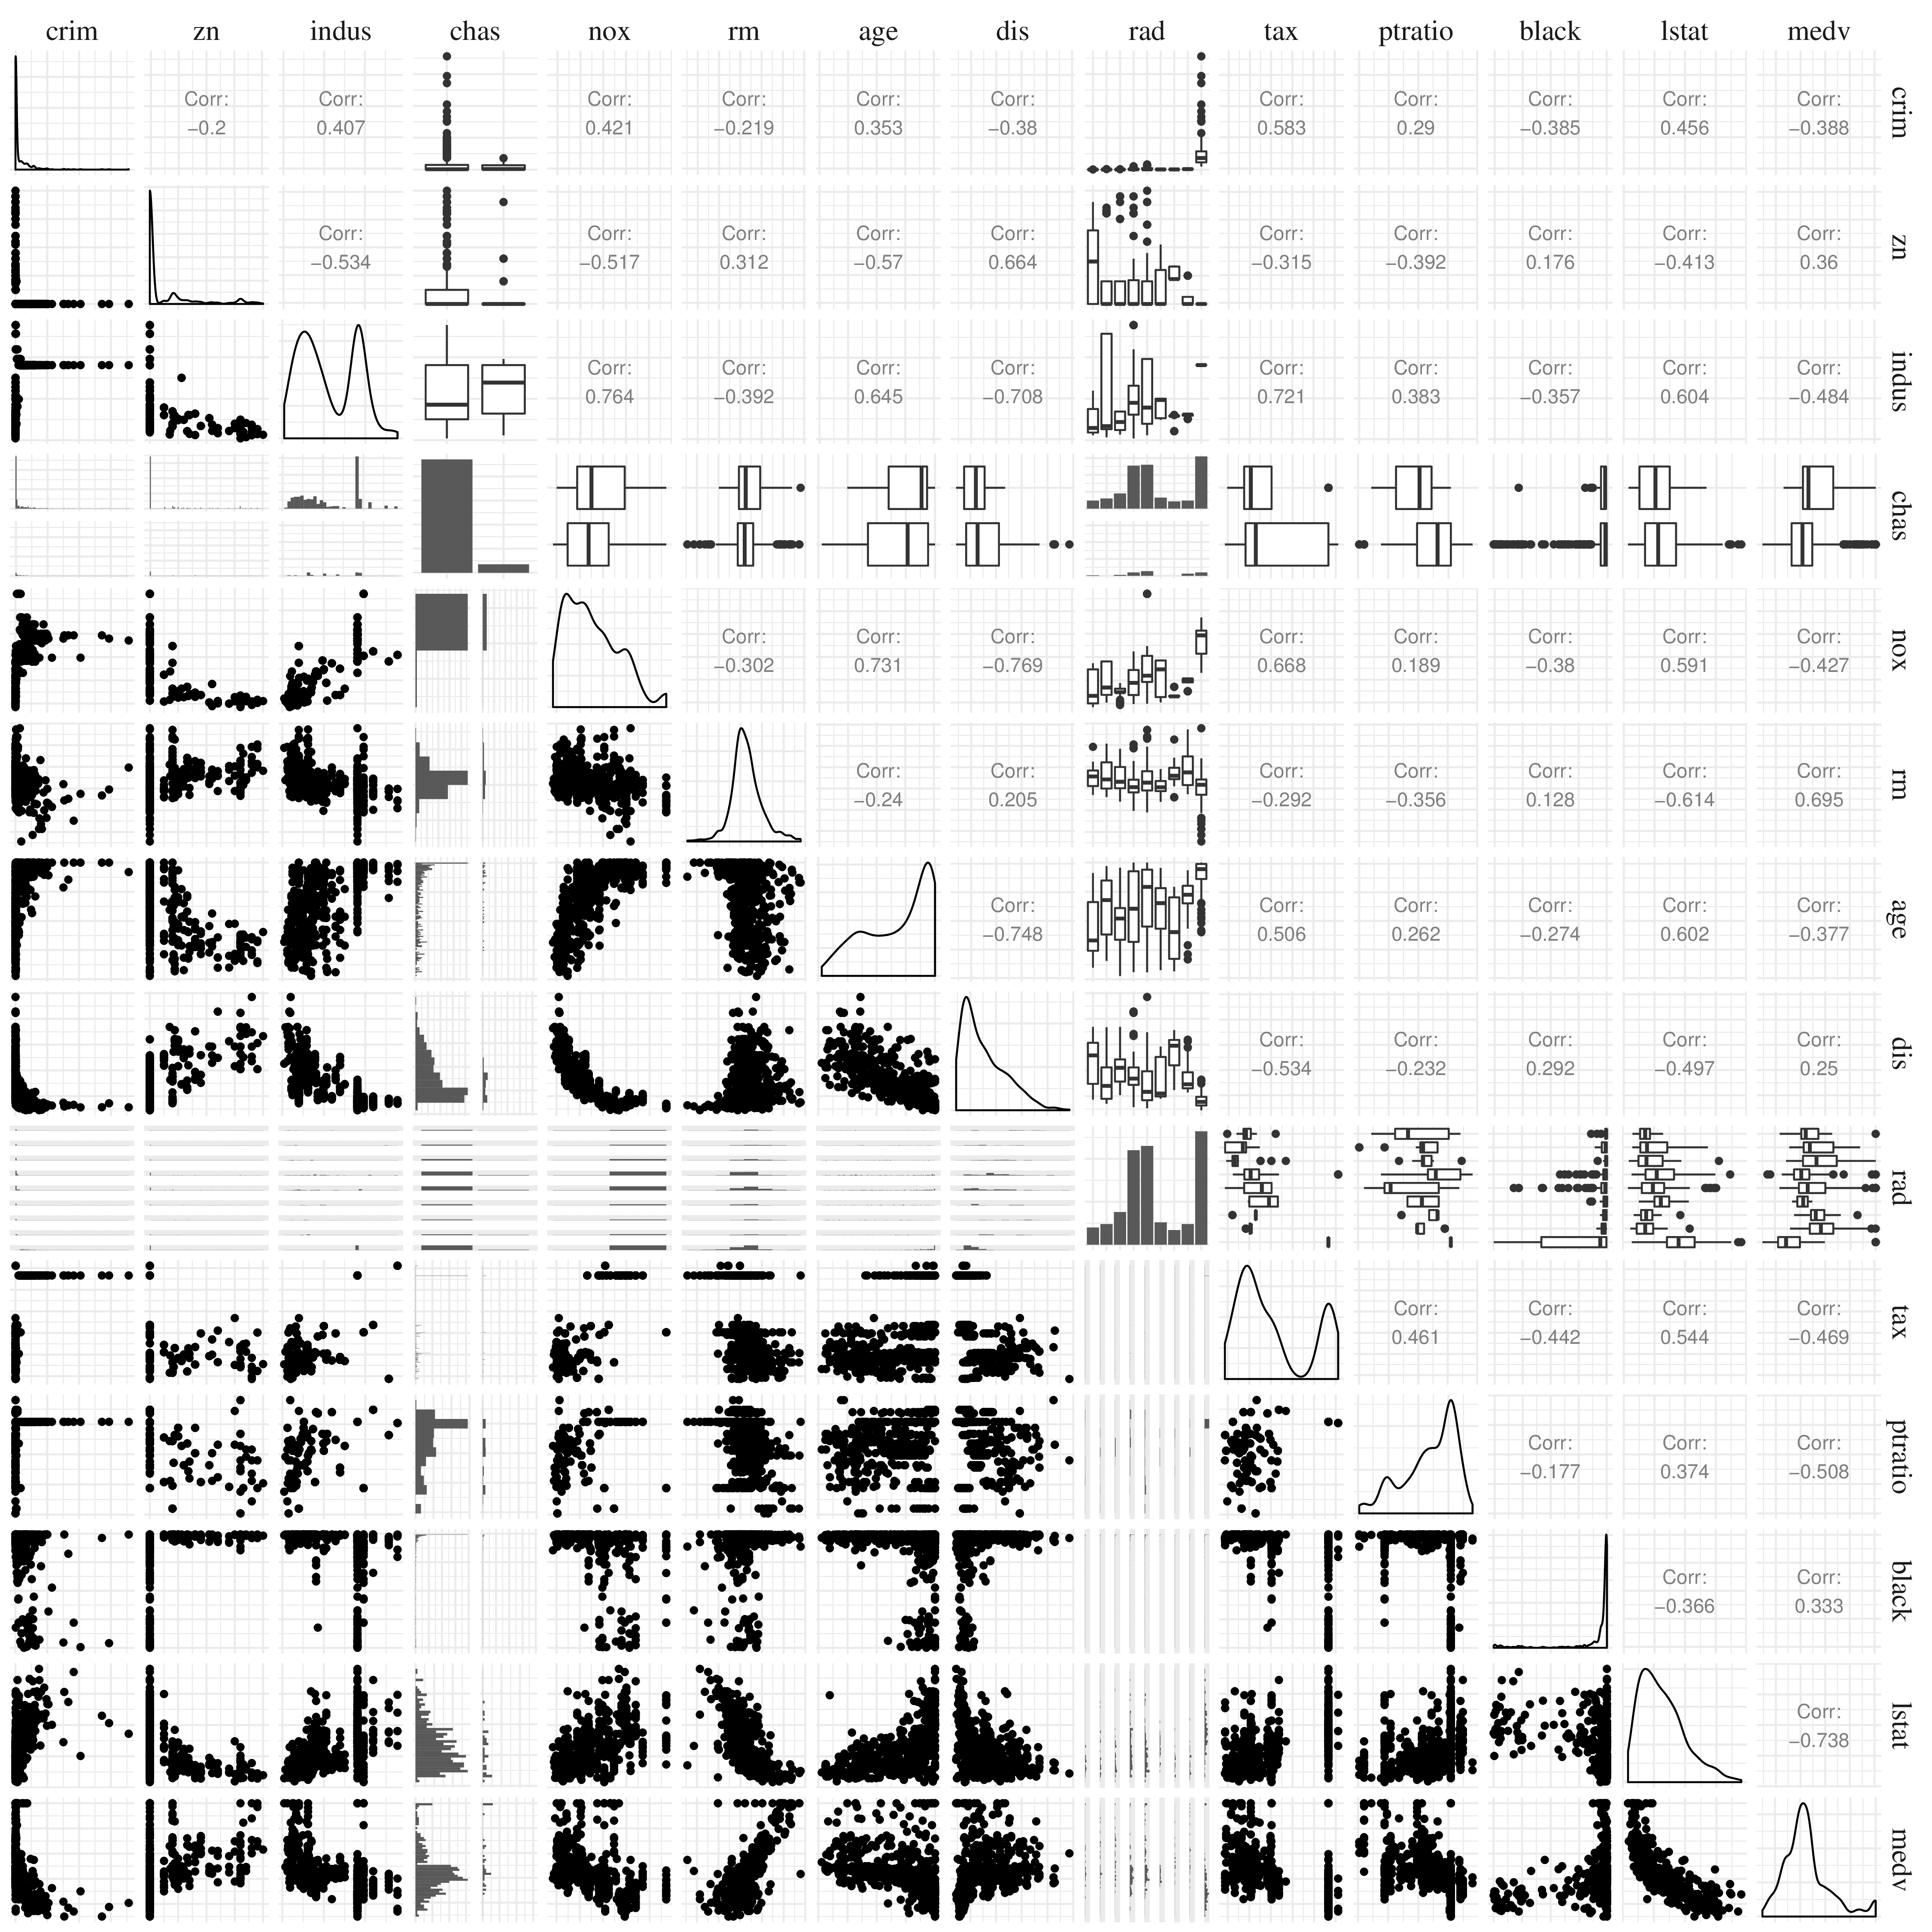
\includegraphics{ISRL_files/figure-latex/ex10b-1.png}
\caption{\label{fig:ex10b}Pairs plot}
\end{figure}

We can see some interesting correlations in this dataset. For exemple, the mean distances to five Boston employement has a correlation of -0.77 with the nitrogen oxides concentration. Or, the lower status of the population are related to the average number of rooms per dwelling (-0.61 for correlation). The variable that are the most related with the crime rate by town is the full-value property-tax rate per \$10,000.

\begin{itemize}
\tightlist
\item
  \emph{Question (c)}
\end{itemize}

The variable \emph{crim} seems to be associated with the variables \emph{tax}, \emph{lstat} and \emph{nox} because they have quite a large correlation with the variable of interest (cf.~previous question).

\begin{itemize}
\tightlist
\item
  \emph{Question (d)}
\end{itemize}

\begin{figure}
\centering
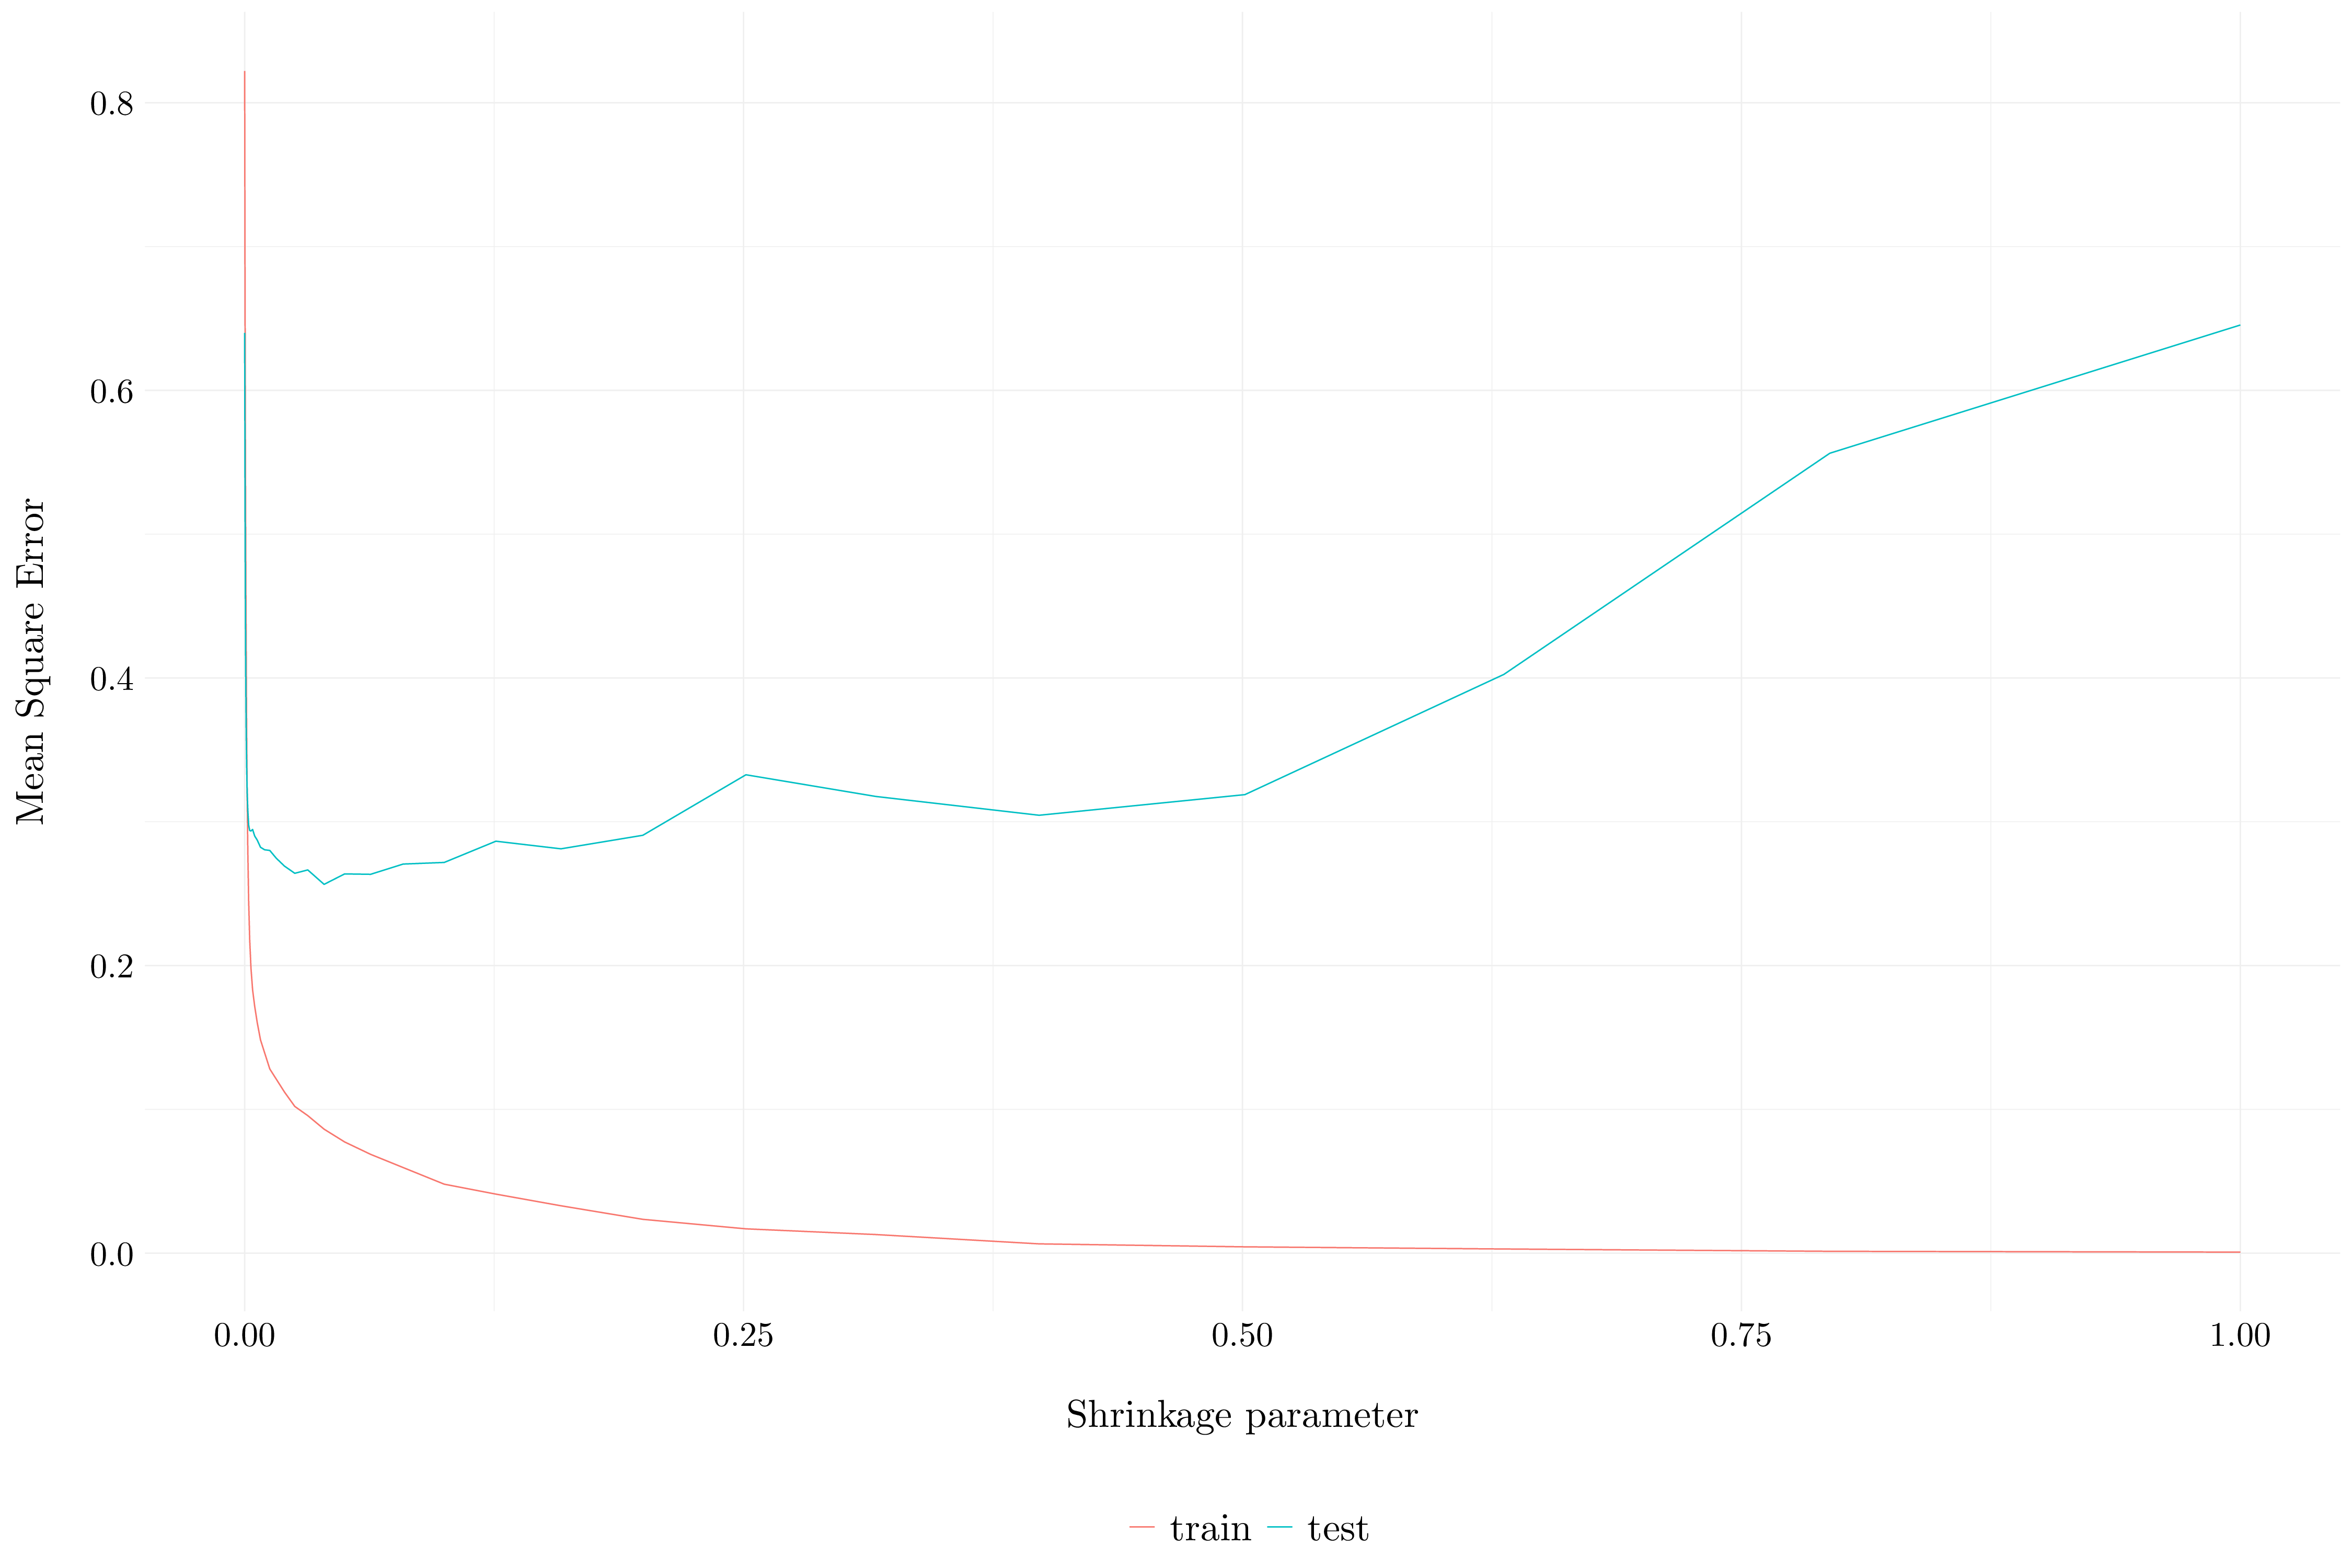
\includegraphics{ISRL_files/figure-latex/ex10d-1.png}
\caption{\label{fig:ex10d}Boxplots of some variables.}
\end{figure}

Half of the suburbs have less than 10\% of crime rates, but for three of them, this rate is greater than 70\%. The range for this variable is very important. The tax rates do not seem to have outliers but the range is also very important. Indeed, the tax can go from under \$200,000 to above \$700,000. Finally, there are some suburbs in Boston that have a very low pupil-teacher ratio compare to the others. However, the range is not very wide.

\begin{itemize}
\tightlist
\item
  \emph{Question (e)}
\end{itemize}

There are 35 suburbs that bound the Charles river.

\begin{itemize}
\tightlist
\item
  \emph{Question (f)}
\end{itemize}

The median pupil-teacher ratio among the towns of Boston is 19.05\%.

\begin{itemize}
\tightlist
\item
  \emph{Question (g)}
\end{itemize}

\begin{Shaded}
\begin{Highlighting}[]
\NormalTok{Boston[}\KeywordTok{which}\NormalTok{(Boston}\OperatorTok{$}\NormalTok{medv }\OperatorTok{==}\StringTok{ }\KeywordTok{min}\NormalTok{(Boston}\OperatorTok{$}\NormalTok{medv)),] }\OperatorTok\StringTok{ }\KeywordTok{print_df}\NormalTok{() }
\end{Highlighting}
\end{Shaded}

crim

zn

indus

chas

nox

rm

age

dis

rad

tax

ptratio

black

lstat

medv

38.3518

0

18.1

FALSE

0.693

5.453

100

1.4896

24

666

20.2

396.90

30.59

5

67.9208

0

18.1

FALSE

0.693

5.683

100

1.4254

24

666

20.2

384.97

22.98

5

Two suburbs share the lowest median value of owner-occupied homes in \$1000s. They have pretty the same values for the other predictors (except maybe for the crime rate).

\begin{itemize}
\tightlist
\item
  \emph{Question (h)}
\end{itemize}

There are 64 suburbs with an average of number of rooms per dwelling larger than 7 and 13 with more than 8.

\begin{Shaded}
\begin{Highlighting}[]
\NormalTok{Boston[}\KeywordTok{which}\NormalTok{(Boston}\OperatorTok{$}\NormalTok{rm }\OperatorTok{>}\StringTok{ }\DecValTok{8}\NormalTok{),] }\OperatorTok\StringTok{ }\KeywordTok{print_df}\NormalTok{()}
\end{Highlighting}
\end{Shaded}

crim

zn

indus

chas

nox

rm

age

dis

rad

tax

ptratio

black

lstat

medv

0.12083

0

2.89

FALSE

0.4450

8.069

76.0

3.4952

2

276

18.0

396.90

4.21

38.7

1.51902

0

19.58

TRUE

0.6050

8.375

93.9

2.1620

5

403

14.7

388.45

3.32

50.0

0.02009

95

2.68

FALSE

0.4161

8.034

31.9

5.1180

4

224

14.7

390.55

2.88

50.0

0.31533

0

6.20

FALSE

0.5040

8.266

78.3

2.8944

8

307

17.4

385.05

4.14

44.8

0.52693

0

6.20

FALSE

0.5040

8.725

83.0

2.8944

8

307

17.4

382.00

4.63

50.0

0.38214

0

6.20

FALSE

0.5040

8.040

86.5

3.2157

8

307

17.4

387.38

3.13

37.6

0.57529

0

6.20

FALSE

0.5070

8.337

73.3

3.8384

8

307

17.4

385.91

2.47

41.7

0.33147

0

6.20

FALSE

0.5070

8.247

70.4

3.6519

8

307

17.4

378.95

3.95

48.3

0.36894

22

5.86

FALSE

0.4310

8.259

8.4

8.9067

7

330

19.1

396.90

3.54

42.8

0.61154

20

3.97

FALSE

0.6470

8.704

86.9

1.8010

5

264

13.0

389.70

5.12

50.0

0.52014

20

3.97

FALSE

0.6470

8.398

91.5

2.2885

5

264

13.0

386.86

5.91

48.8

0.57834

20

3.97

FALSE

0.5750

8.297

67.0

2.4216

5

264

13.0

384.54

7.44

50.0

3.47428

0

18.10

TRUE

0.7180

8.780

82.9

1.9047

24

666

20.2

354.55

5.29

21.9

\hypertarget{literature}{%
\chapter{Literature}\label{literature}}

Here is a review of existing methods.

\hypertarget{methods}{%
\chapter{Methods}\label{methods}}

We describe our methods in this chapter.

\hypertarget{applications}{%
\chapter{Applications}\label{applications}}

Some \emph{significant} applications are demonstrated in this chapter.

\hypertarget{example-one}{%
\section{Example one}\label{example-one}}

\hypertarget{example-two}{%
\section{Example two}\label{example-two}}

\hypertarget{final-words}{%
\chapter{Final Words}\label{final-words}}

We have finished a nice book.

\bibliography{book.bib,packages.bib}


\end{document}
